\subsection{题目描述}
\noindent
Consider the Poisson equation:
\[
    \nabla^2 \varphi(x, y) = -\frac{\rho(x, y)}{\varepsilon_0}
\]
from electrostatics on a rectangular geometry with \(x \in [0, L_x]\) and \(y \in [0, L_y]\). Write a program that solves this equation using the relaxation method and test your program with the following cases:

\noindent
(a) \(\rho(x, y) = 0\), \(\varphi(0, y) = \varphi(L_x, y) = \varphi(x, 0) = 0\), \(\varphi(x, L_y) = 1 \, \text{V}\),
\(L_x = 1 \, \text{m}\), and \(L_y = 1.5 \, \text{m}\);

\noindent
(b) \(\frac{\rho(x, y)}{\varepsilon_0} = 1 \, \text{V/m}^2\), \(\varphi(0, y) = \varphi(L_x, y) = \varphi(x, 0) = \varphi(x, L_y) = 0\), and \(L_x = L_y = 1 \, \text{m}\).


\subsection{程序描述}
本程序支持在题示两种案例与自定义案例(指定矩形区域大小、求解参数、均匀源项与第一类边界条件,即四周电势)下的求解,并内置了解析解的计算,以便于对比。其中对于案例 (a) ,即无源电荷,三边接地,齐次解为:
\[
    \phi_h(x,y) = \frac{4V_0}{\pi} \sum_{n=1,3,5,\dots}^{N} \frac{1}{n} \sin\left(\frac{n\pi x}{L_x}\right) \frac{\sinh\left(\frac{n\pi y}{L_x}\right)}{\sinh\left(\frac{n\pi L_y}{L_x}\right)}
\]
考虑到$sinh$函数在$\approx \exp( 700)$会数值溢出,在$N$达到$N_{approx}$时进行指数近似
\[
    \frac{\sinh\left(\frac{n\pi y}{L_x}\right)}{\sinh\left(\frac{n\pi L_y}{L_x}\right)}
    \approx \exp\left(\frac{n\pi (y-L_y)}{L_x} \right)
\]
对于案例 (b) ,即均匀源电荷,四边接地,满足接地条件与均匀源项的特解为:
\[
    \phi_p(x,y) = \sum_{n=1,3,5,\dots}^{N} \sum_{m=1,3,5,\dots}^{M} \frac{16 \rho}{\varepsilon_0 \pi^2 n m \left( \left( \frac{n\pi}{L_x} \right)^2 + \left( \frac{m\pi}{L_y} \right)^2 \right)} \sin\left( \frac{n\pi x}{L_x} \right) \sin\left( \frac{m\pi y}{L_y} \right)
\]
理论上这个级数不是绝对收敛的,且只能计算到一定的阶数,应当采用黎曼求和的对角线求和次序,但在最初的代码中偷懒直接使用了内外for循环,结果是解析解与误差图中x,y方向不对称。但在测试中发现,这种不对称的周期正好与截断项数$N,M$可以对应,因此保留了这个小bug,恰可以增加一重误差图的物理含义检验。
对于自定义案例,根据用户指定的边界条件,相应的解析解只需计算四个边界条件(需要改变自变量进行旋转)对应的齐次解$\phi^i_h(x,y)$进行叠加,再加上均匀源项的接地特解$\phi_p(x,y)$即可
\[
    \phi(x,y) = \sum_{i=1}^{4} \phi_h^i(x,y) + \phi_p(x,y)
\]

在求解器\texttt{PoissonSolver}类中,内置了Jacobi, Gauss-Seidel, SOR三种迭代方法,用户可以通过\texttt{method}参数选择。它们的算法细节将在伪代码中详细介绍。其中SOR的松弛因子$\omega$根据输入参数由\texttt{get\_optimal\_omega}方法自动计算,采用的公式来自\textit{Numeric Recipes}(2nd ed.)的第19.5节,即
\[\omega=\frac2{1+\sqrt{1-\rho_{\mathrm{Jacobi}}^2}}\]
其中$\rho_{\mathrm{Jacobi}}$为Jacobi方法的谱半径
\[\rho_\text{Jacobi}=\frac{\cos\frac\pi {N_x}+\left(\frac{\Delta x}{\Delta y}\right)^2\cos\frac\pi {N_y}}{1+\left(\frac{\Delta x}{\Delta y}\right)^2}\]
在等间距正方形大网格中化为课件中的近似表达式
\(\omega \simeq \frac{2}{1+\pi / L}\)
实际测试表明该因子选取大幅加快收敛速度,赞!

请在\texttt{Problem\_1/src}目录下运行\ccmd{python -u poisson.py},需安装辅助计算的\texttt{numpy}库与绘图用的\texttt{matplotlib}库。程序从用户输入获取求解案例及参数之后,将首先输出三种方法的迭代动画(步数过多时抽取最多100帧进行展示),随后绘制三者的收敛曲线,即每步最大变化量随步数的变化。最后输出计算结果及与解析解的对比图,以及计算误差图,详见下文的结果示例。
\subsection{伪代码}
Powered by \href{https://chatgpt.com/g/g-xJJAA2awf-latex-pseudocode-generator}{\LaTeX \ pseudocode generator}

\begin{algorithm}[H]
    \SetAlgoLined
    \KwIn{$\phi$ (potential matrix), \texttt{tolerance}, \texttt{max\_iter}}
    \KwOut{$\phi$ (updated potential matrix)}
    \BlankLine

    \SetKwData{MaxChange}{max\_change}
    \SetKwData{Denom}{denom}
    \SetKwData{Dx2}{dx2}
    \SetKwData{Dy2}{dy2}

    $dx^2 \leftarrow dx^2,\ dy^2 \leftarrow dy^2,\ \Denom \leftarrow 2 \times (dx^2 + dy^2)$ \tcp*[r]{Precompute constants}

    \For{$it \leftarrow 1$ \KwTo \texttt{max\_iter}}{
        $\phi_{\text{new}} \leftarrow \phi$ \tcp*[r]{Create a copy for new updates}

        \For{$i \leftarrow 1$ \KwTo $N_x - 2$}{
            \For{$j \leftarrow 1$ \KwTo $N_y - 2$}{
                $\phi_{\text{new}}[i,j] \leftarrow \frac{
                        (\phi[i+1,j] + \phi[i-1,j]) \times dy^2 + (\phi[i,j+1] + \phi[i,j-1]) \times dx^2 + dx^2 \times dy^2 \times \rho_{\epsilon_0}[i,j]
                    }{\Denom}$ \tcp*[r]{Jacobi update}
            }
        }

        \MaxChange $\leftarrow \max(|\phi_{\text{new}} - \phi|)$ \;
        \If{\MaxChange $<$ \texttt{tolerance}}{\Return $\phi_{\text{new}}$ \tcp*[r]{Convergence reached}}

        $\phi \leftarrow \phi_{\text{new}}$ \tcp*[r]{Update for next iteration}
    }

    \Return $\phi$ \tcp*[r]{Return after max iterations}
    \caption{Jacobi Method for Solving Poisson's Equation}
\end{algorithm}
\begin{algorithm}[H]
    \SetAlgoLined
    \KwIn{$\phi$ (potential matrix), \texttt{tolerance}, \texttt{max\_iter}}
    \KwOut{$\phi$ (updated potential matrix)}
    \BlankLine

    \SetKwData{MaxChange}{max\_change}
    \SetKwData{Denom}{denom}
    \SetKwData{Dx2}{dx2}
    \SetKwData{Dy2}{dy2}

    $dx^2 \leftarrow dx^2,\ dy^2 \leftarrow dy^2,\ \Denom \leftarrow 2 \times (dx^2 + dy^2)$ \tcp*[r]{Precompute constants}

    \For{$it \leftarrow 1$ \KwTo \texttt{max\_iter}}{
        \MaxChange $\leftarrow 0$ \tcp*[r]{Reset max change for this iteration}

        \For{$i \leftarrow 1$ \KwTo $N_x - 2$}{
            \For{$j \leftarrow 1$ \KwTo $N_y - 2$}{
                $\phi_{\text{old}} \leftarrow \phi[i,j]$ \;
                $\phi[i,j] \leftarrow \frac{
                        (\phi[i+1,j] + \phi[i-1,j]) \times dy^2 + (\phi[i,j+1] + \phi[i,j-1]) \times dx^2 + dx^2 \times dy^2 \times \rho_{\epsilon_0}[i,j]
                    }{\Denom}$ \tcp*[r]{Gauss-Seidel update}
                \MaxChange $\leftarrow \max(\MaxChange, |\phi[i,j] - \phi_{\text{old}}|)$ \tcp*[r]{Track max change}
            }
        }

        \If{\MaxChange $<$ \texttt{tolerance}}{\Return $\phi$ \tcp*[r]{Convergence reached}}
    }

    \Return $\phi$ \tcp*[r]{Return after max iterations}
    \caption{Gauss-Seidel Method for Solving Poisson's Equation}
\end{algorithm}
\begin{algorithm}[H]
    \SetAlgoLined
    \KwIn{$\phi$ (potential matrix), $\omega$ (relaxation factor), \texttt{tolerance}, \texttt{max\_iter}}
    \KwOut{$\phi$ (updated potential matrix)}
    \BlankLine

    \SetKwData{MaxChange}{max\_change}
    \SetKwData{Denom}{denom}
    \SetKwData{Dx2}{dx2}
    \SetKwData{Dy2}{dy2}

    $dx^2 \leftarrow dx^2,\ dy^2 \leftarrow dy^2,\ \Denom \leftarrow 2 \times (dx^2 + dy^2)$ \tcp*[r]{Precompute constants}

    \For{$it \leftarrow 1$ \KwTo \texttt{max\_iter}}{
        \MaxChange $\leftarrow 0$ \tcp*[r]{Reset max change for this iteration}

        \For{$i \leftarrow 1$ \KwTo $N_x - 2$}{
            \For{$j \leftarrow 1$ \KwTo $N_y - 2$}{
                $\phi_{\text{old}} \leftarrow \phi[i,j]$ \;
                $\phi_{\text{new}} \leftarrow \frac{
                        (\phi[i+1,j] + \phi[i-1,j]) \times dy^2 + (\phi[i,j+1] + \phi[i,j-1]) \times dx^2 + dx^2 \times dy^2 \times \rho_{\epsilon_0}[i,j]
                    }{\Denom}$ \tcp*[r]{Standard update}
                $\phi[i,j] \leftarrow (1 - \omega) \cdot \phi_{\text{old}} + \omega \cdot \phi_{\text{new}}$ \tcp*[r]{SOR update}
                \MaxChange $\leftarrow \max(\MaxChange, |\phi[i,j] - \phi_{\text{old}}|)$ \tcp*[r]{Track max change}
            }
        }

        \If{\MaxChange $<$ \texttt{tolerance}}{\Return $\phi$ \tcp*[r]{Convergence reached}}
    }

    \Return $\phi$ \tcp*[r]{Return after max iterations}
    \caption{SOR Method for Solving Poisson's Equation}
\end{algorithm}
\subsection{结果示例}
\subsubsection{Case (a):无源电荷,三边接地}
\begin{figure}[H]
    \centering
    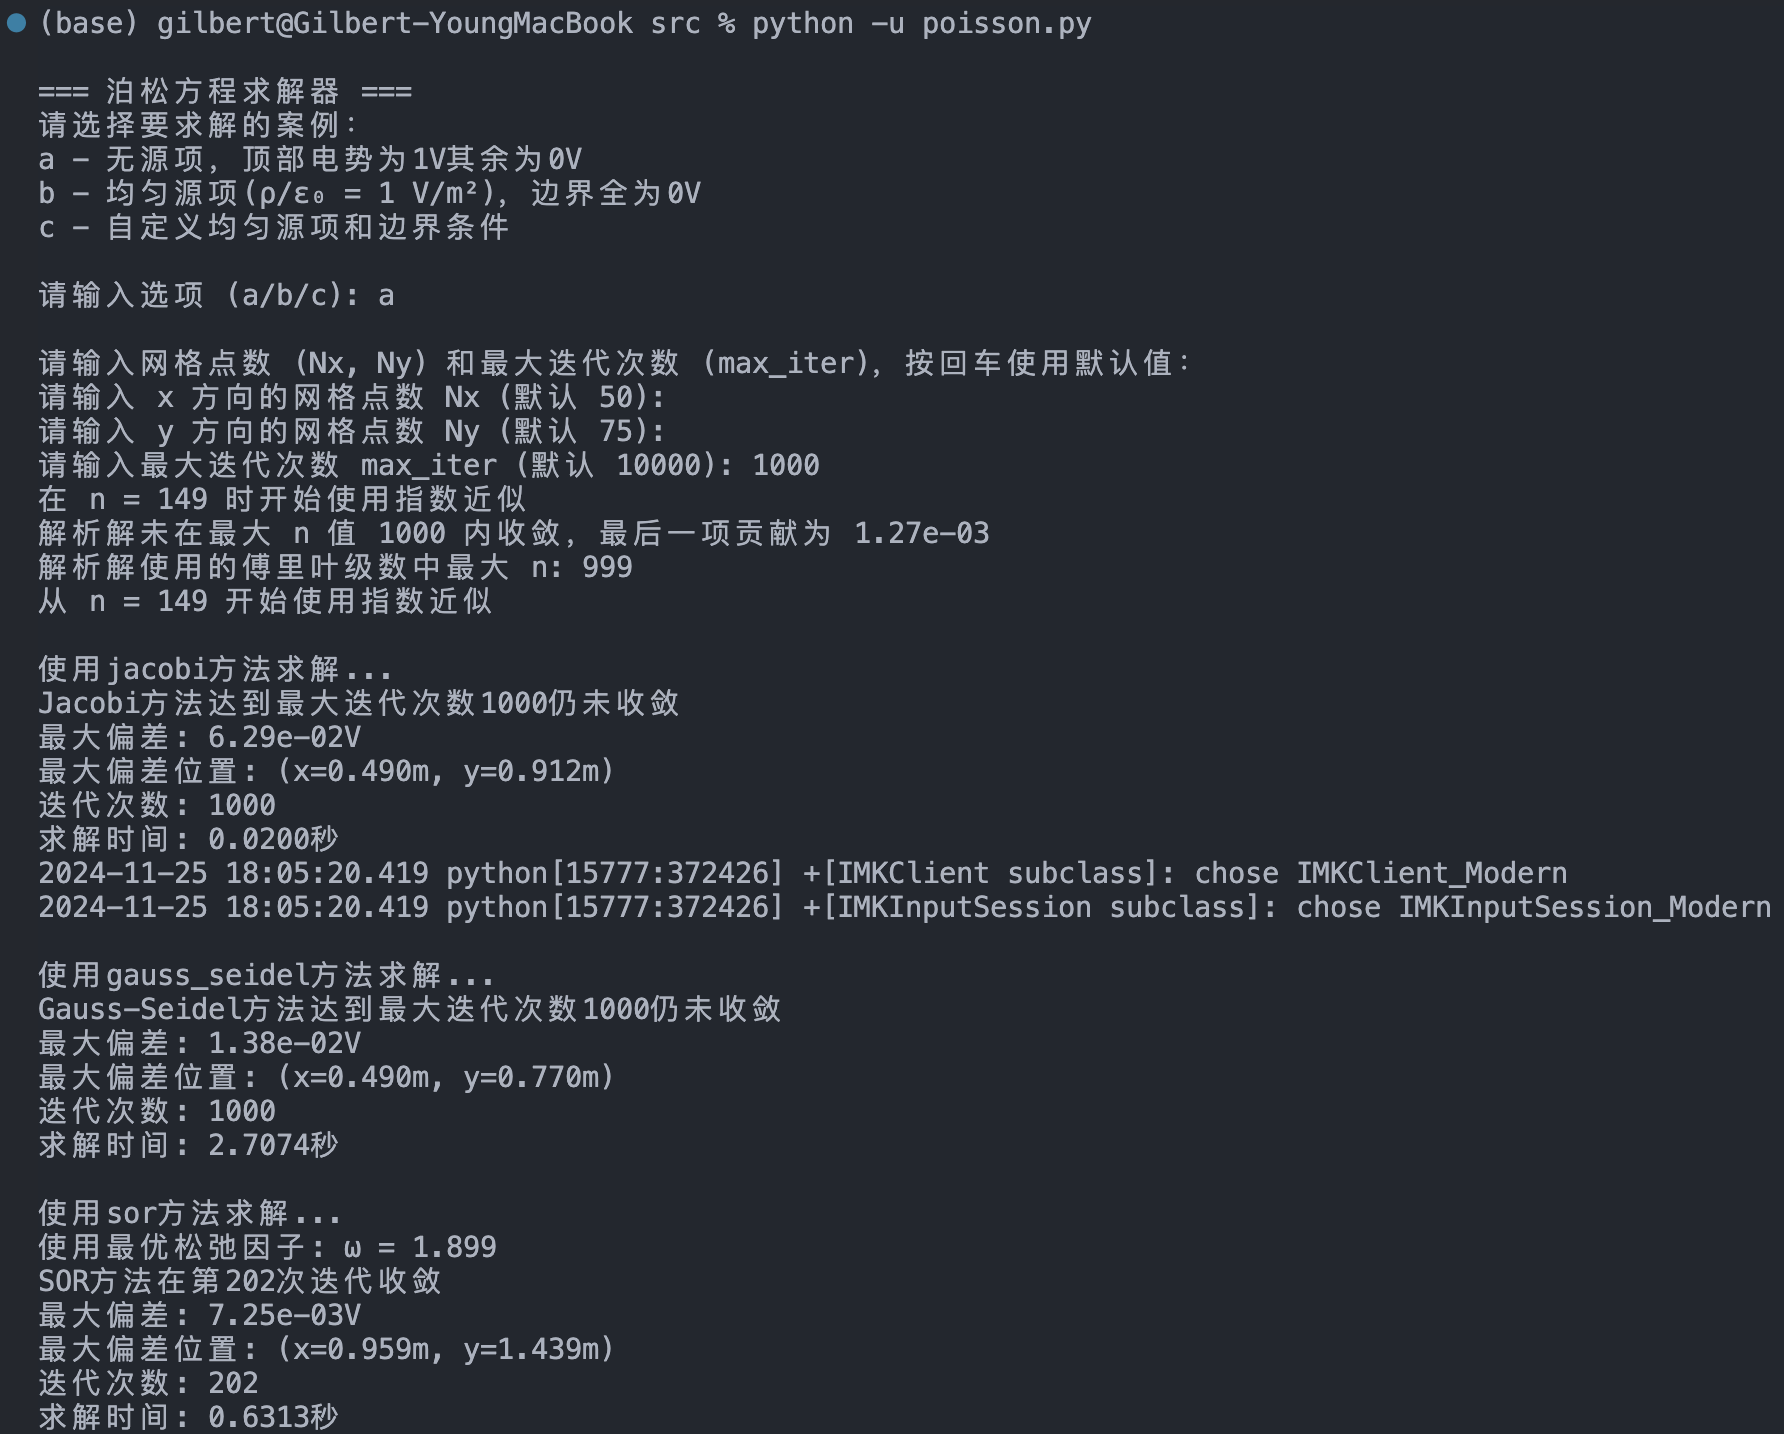
\includegraphics[width=1.0\textwidth]{Problem_1/figs/a_terminal.png}
    \caption{(a):终端输出}
\end{figure}
本次测试特地将最大迭代次数截断在1000,以测试三种方式的精度与收敛速度。可以看到最终与解析解的最大误差比较中,Jacobi方法的误差最大,而Gauss-Seidel方法的误差较小,SOR方法的误差最小,且在第202步便已收敛至指定精度。在耗时方面,Jacobi因为不需要使用实时更新的$\phi$,可以进行多线程并行,所以耗时反而最短,而Gauss-Seidel方法(隐式)因为需要使用新的$\phi$,耗时最长,SOR方法介于两者之间,虽不能并行,但收敛速度最快。

在输出的误差比较图中,Jacobi与Gauss-Seidel方法的误差图形状相似,最大偏差点均在中心处,但误差更小,而SOR方法几乎没有偏差,最大偏差点在硬性边界条件的不连续处,这非程序本身的问题。\textbf{在运行动画时}将能更直观展现迭代过程,SOR的更新更为迅速且方向准确。
\begin{figure}[H]
    \centering
    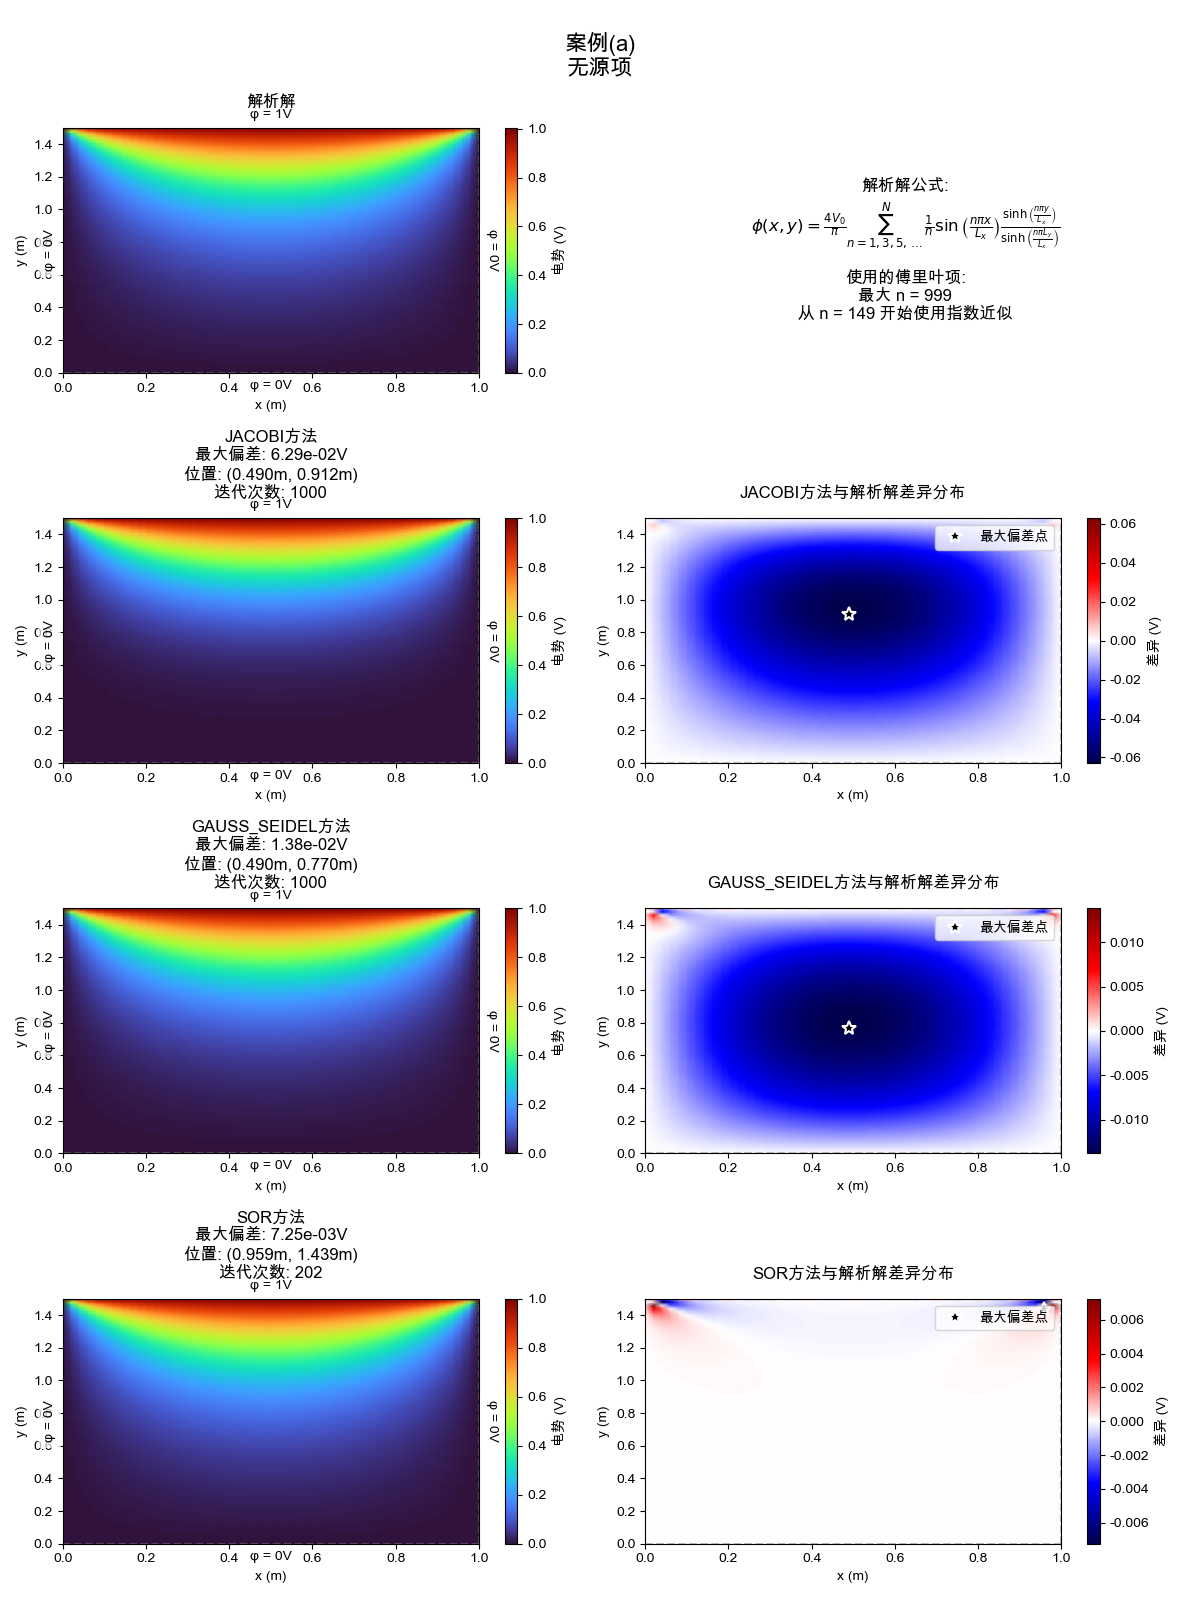
\includegraphics[width=0.9\textwidth]{Problem_1/figs/a_result.png}
    \caption{(a):计算结果及对比}
\end{figure}

\begin{figure}[H]
    \centering
    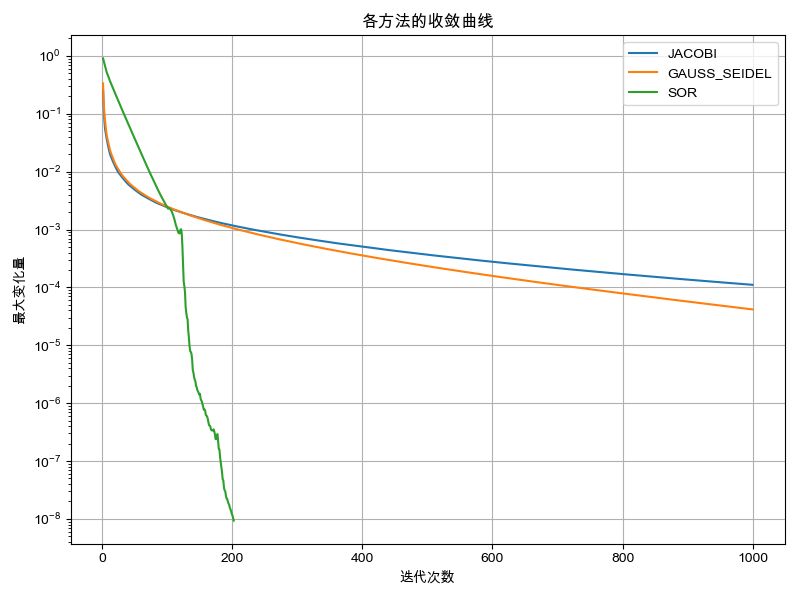
\includegraphics[width=1.0\textwidth]{Problem_1/figs/a_convergence.png}
    \caption{(a):收敛曲线对比}
\end{figure}
收敛曲线的趋势并不完全如课件上的
\[
    r \simeq
    \begin{cases}
        \frac{1}{2}pL^2 & \text{for Jacobi's method},                       \\
        \frac{1}{4}pL^2 & \text{for the Gauss-Seidel method},               \\
        \frac{1}{3}pL   & \text{for SOR with } \omega \simeq 2/(1 + \pi/L).
    \end{cases}
\]
不过线性趋势与二次趋势还是大概可以看出来。最初版本的程序使用上式预测收敛次数的功能也删去了,看上去SOR的收敛比预期更为迅猛。
\subsubsection{Case (b):均匀源电荷,四边接地}
\begin{figure}[H]
    \centering
    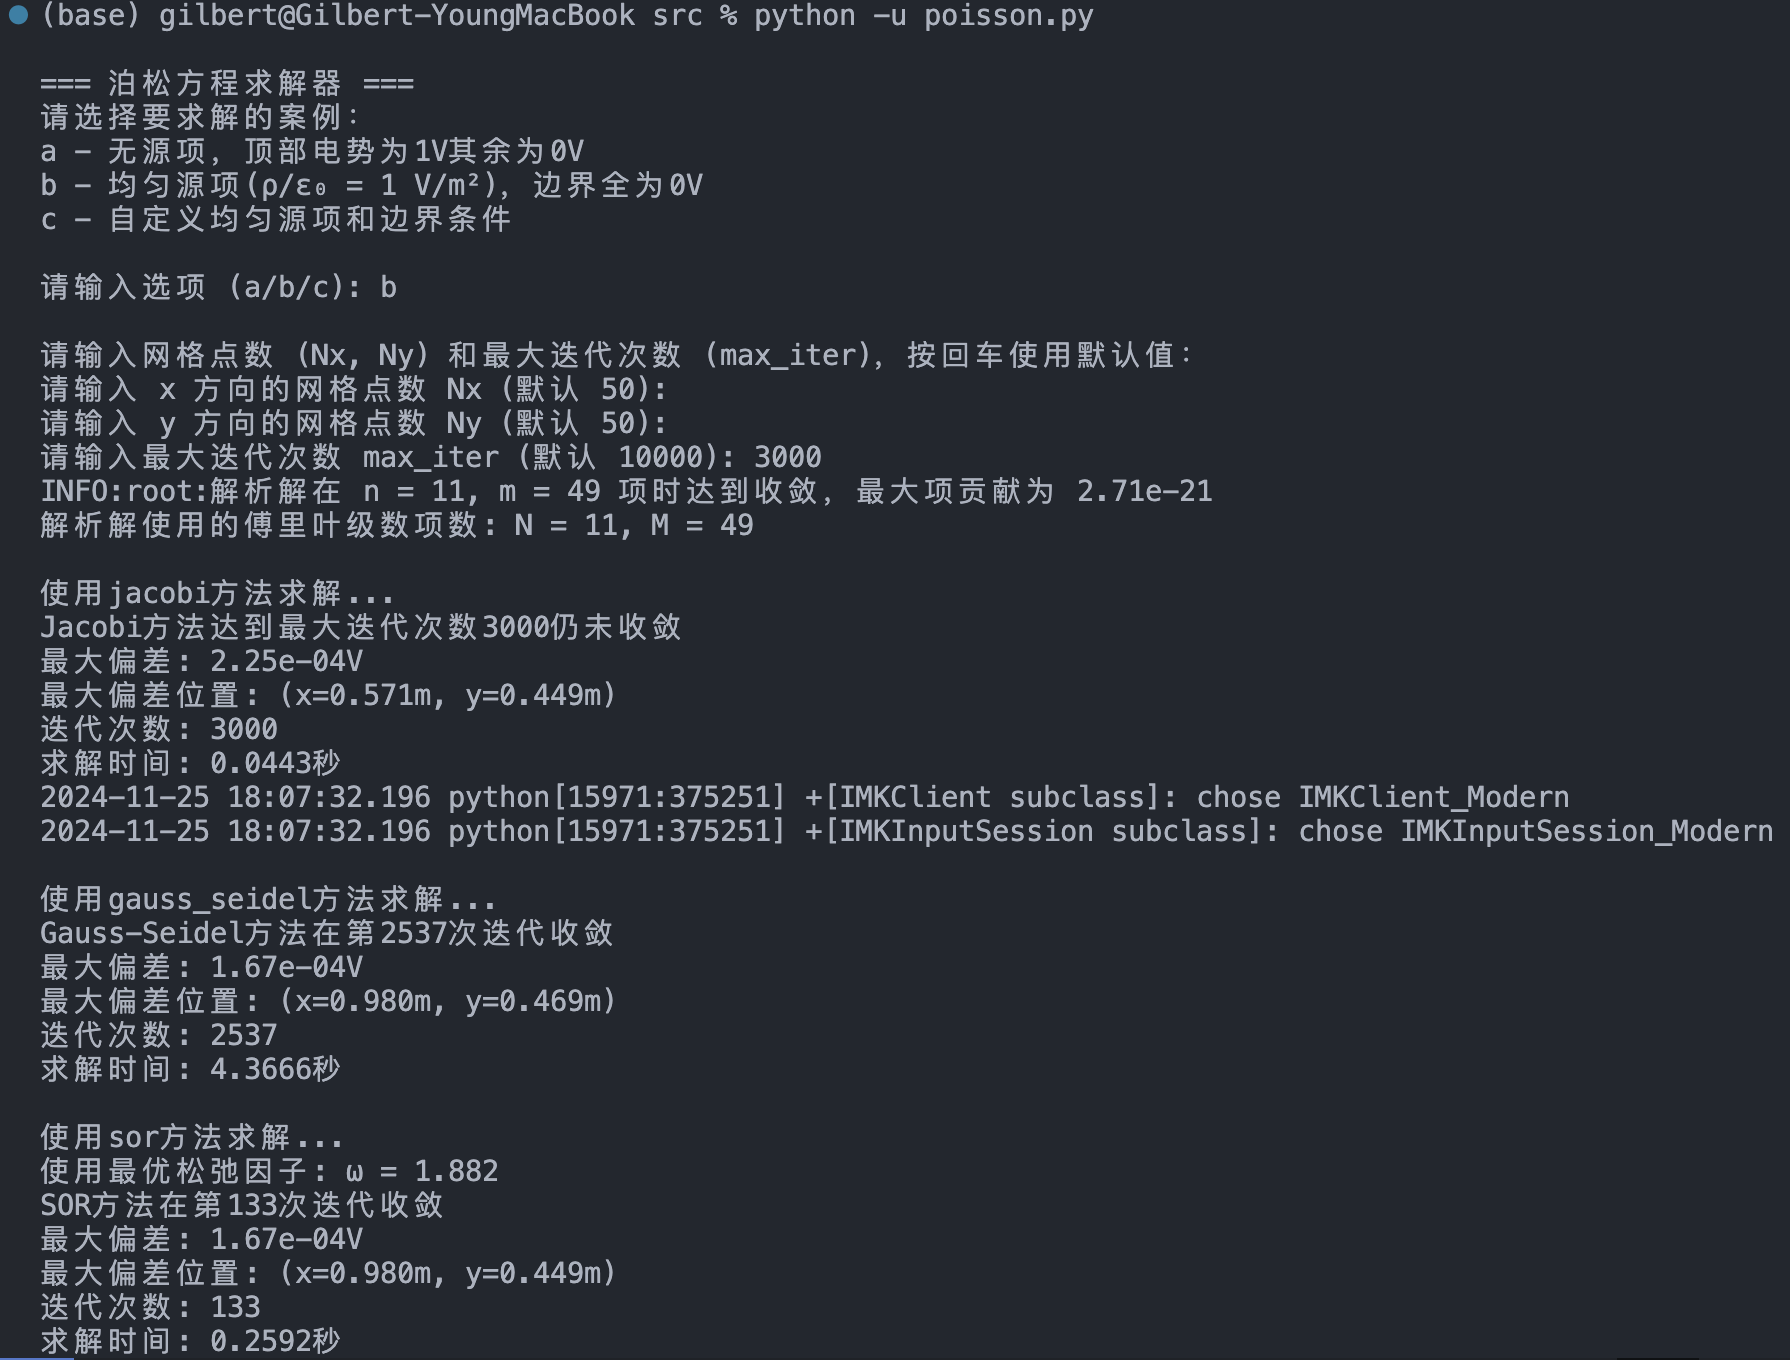
\includegraphics[width=1.0\textwidth]{Problem_1/figs/b_terminal.png}
    \caption{(b):终端输出}
\end{figure}
本案例Jacobi在3000次迭代中都为收敛,Gauss-Seidel方法在第2537次迭代侥幸收敛,而SOR方法在第133次迭代便收敛至指定精度。

比较有意思的是下面的误差比较图,在x方向出现了明显的周期性,且可以在下面两幅子图中验证,该条纹周期恰与上方显示的解析解x方向级数截断$N$对应,表明该误差是解析解截断导致,验证\textbf{前文所述}的,未按照对角线法则计算的级数收敛问题。
\begin{figure}[H]
    \centering
    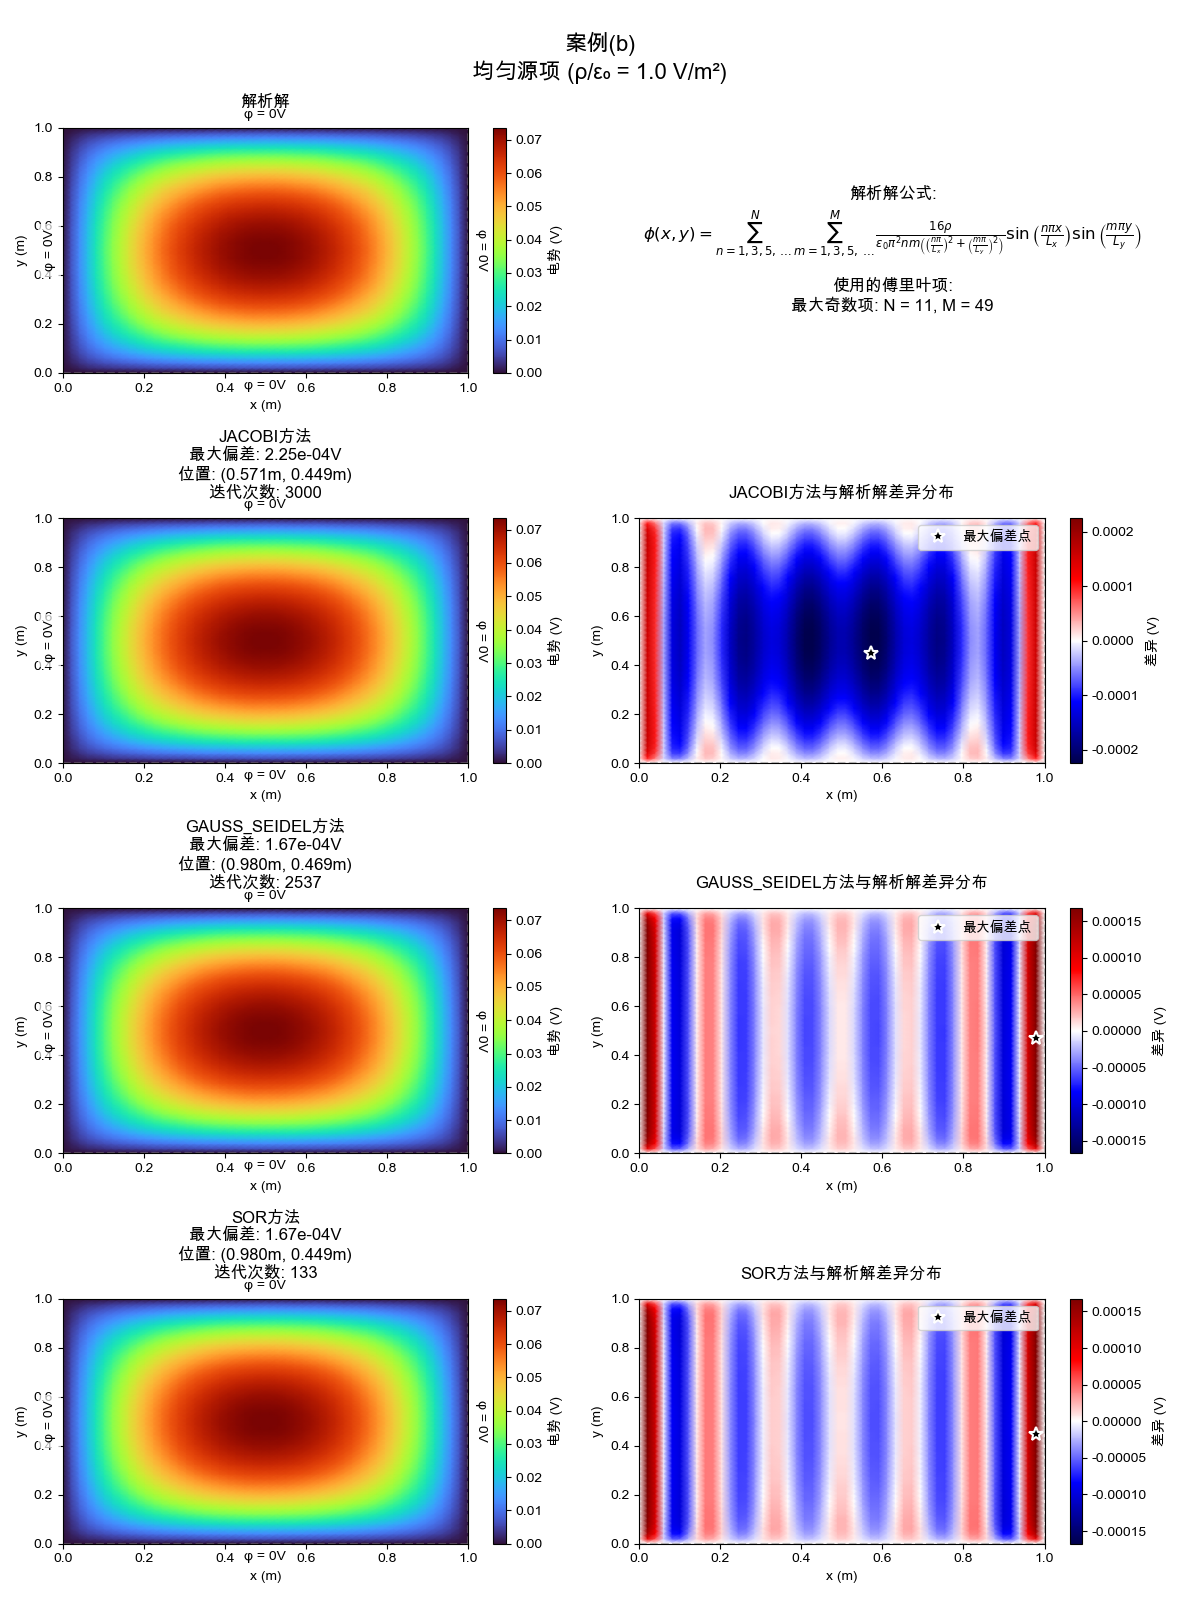
\includegraphics[width=0.9\textwidth]{Problem_1/figs/b_result.png}
    \caption{(b):计算结果及对比}
\end{figure}

\begin{figure}[H]
    \centering
    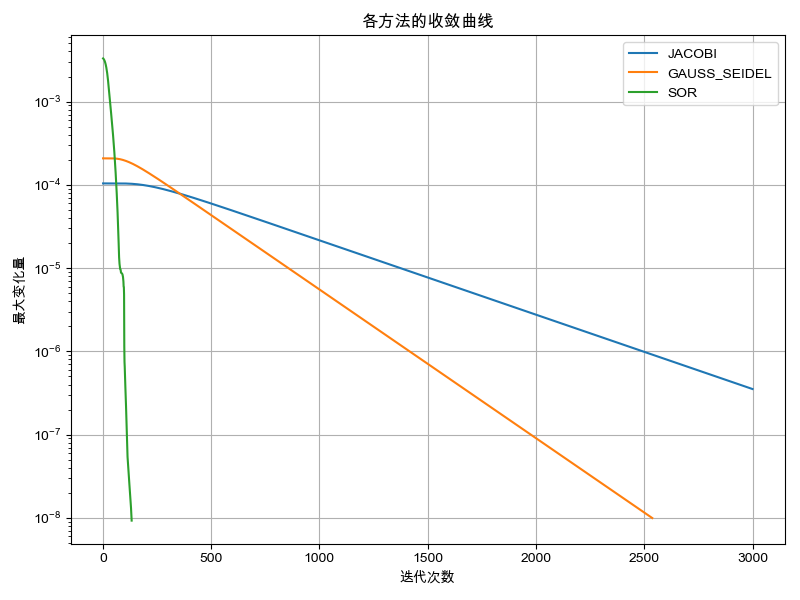
\includegraphics[width=1.0\textwidth]{Problem_1/figs/b_convergence.png}
    \caption{(b):收敛曲线对比}
\end{figure}
此次收敛速度方面,仍是SOR大获全胜,不过尚不清楚其余两种方法的起始点收敛曲线凹凸性起源。
\subsubsection{Case (c):均匀源电荷,自定义边界}
\begin{figure}[H]
    \centering
    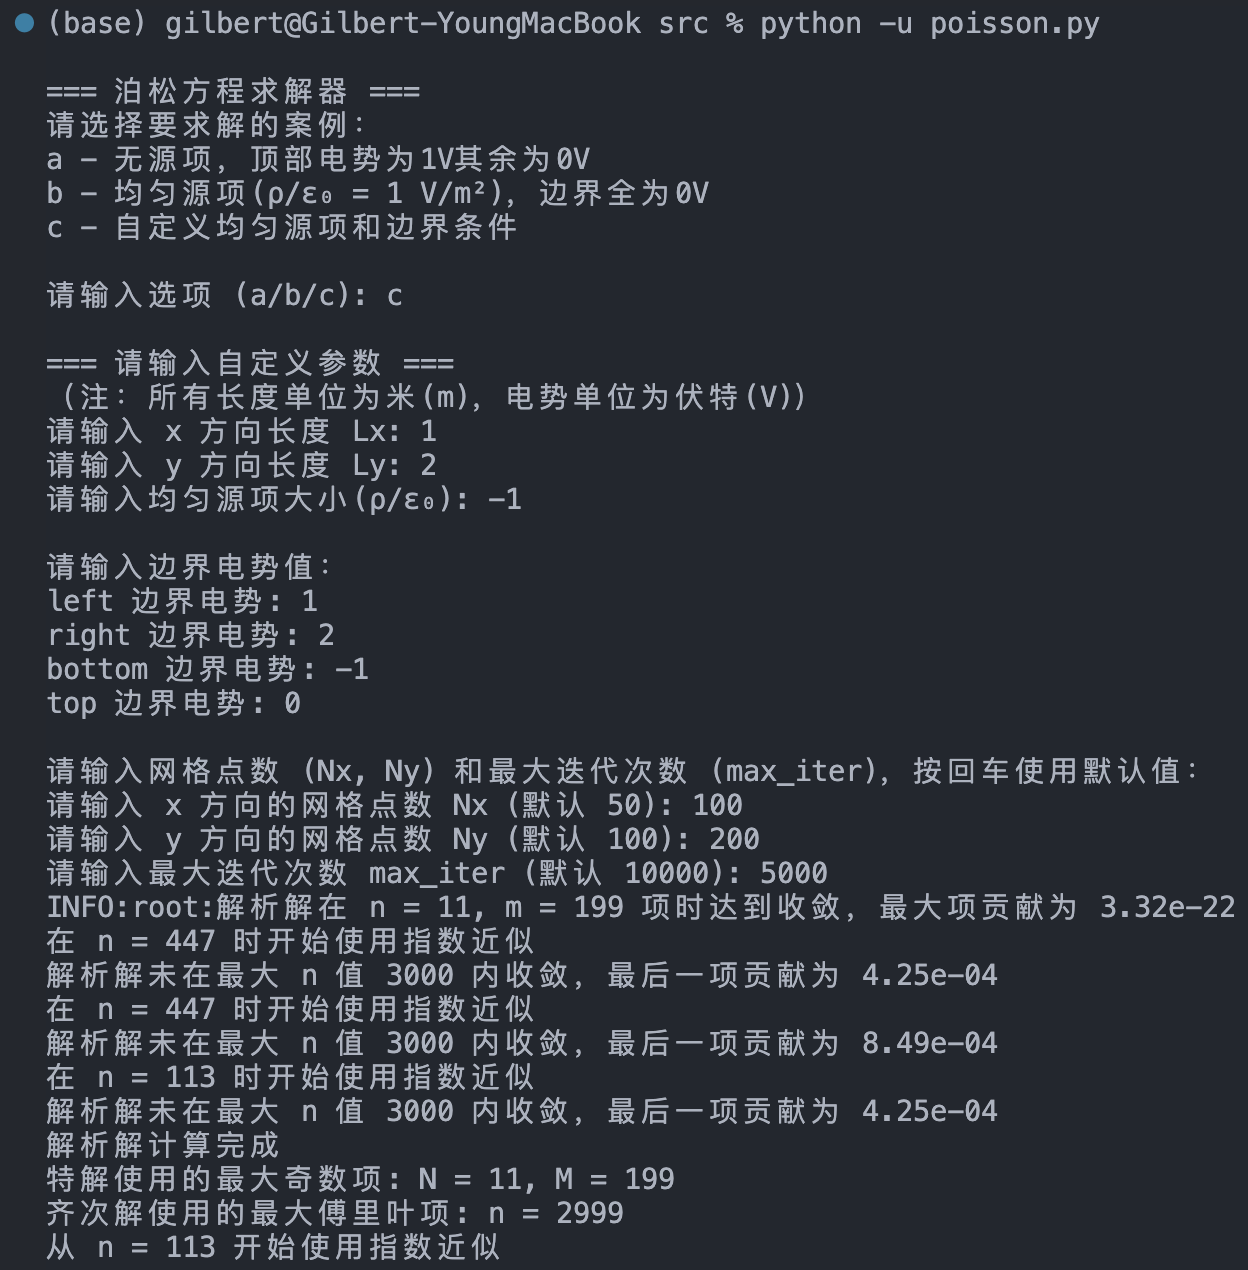
\includegraphics[width=0.5\textwidth]{Problem_1/figs/c_terminal_1.png}
    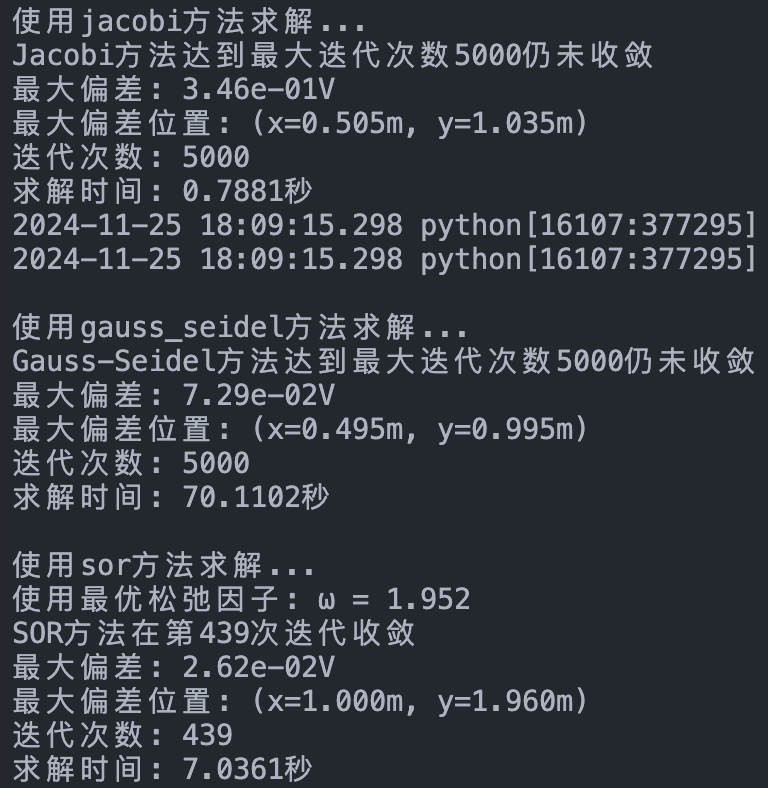
\includegraphics[width=0.5\textwidth]{Problem_1/figs/c_terminal_2.png}
    \caption{(c):终端输出}
\end{figure}
本次在矩形区域添加均匀的负电荷,四周边界条件电势均不相等,程序仍完美执行任务。
\begin{figure}[H]
    \centering
    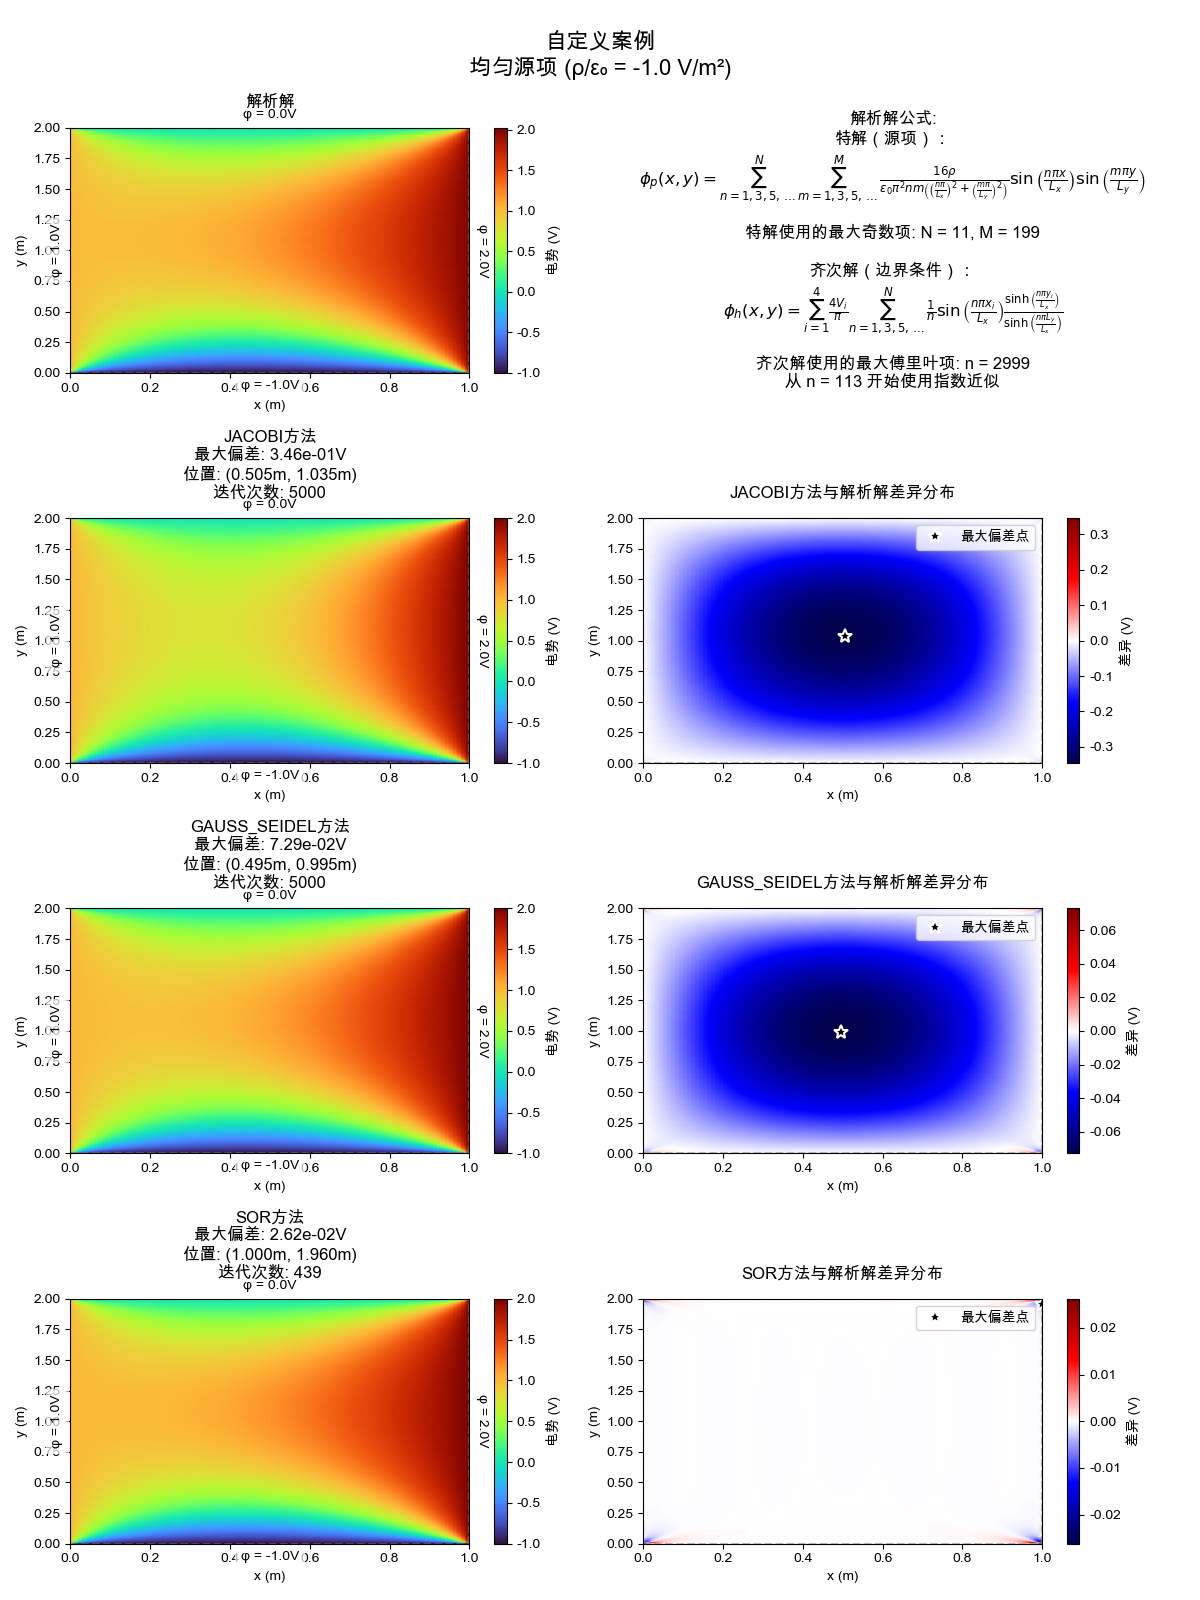
\includegraphics[width=0.9\textwidth]{Problem_1/figs/c_result.png}
    \caption{(c):计算结果及对比}
\end{figure}

\begin{figure}[H]
    \centering
    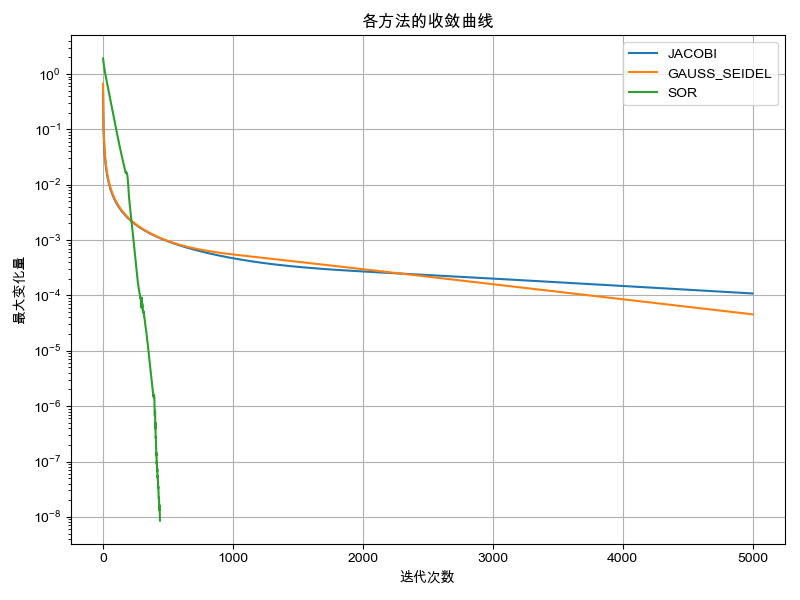
\includegraphics[width=1.0\textwidth]{Problem_1/figs/c_convergence.png}
    \caption{(c):收敛曲线对比}
\end{figure}
